%  !TeX  root  =  user_guide.tex

\chapter{QGIS Server}\label{label_qgisserver}
\index{WMS!QGIS Server}

% when the revision of a section has been finalized,
% comment out the following line:
% \updatedisclaimer

%QGIS Server is an open source WMS 1.3 implementation which, in addition, implements advanced cartographic features for thematic mapping. The QGIS Server is a FastCGI/CGI (Common Gateway Interface) application written in C++ that works together with a webserver (e.g. Apache, Lighttpd). It is funded by the EU projects Orchestra, Sany and the city of Uster in Switzerland.
QGIS Server est un serveur de couches WMS 1.3 open source qui propose également des fonctionnalités avancées de cartographie thématique. Il s'agit d'une application FastCGI/CGI (Common Gateway Interface) écrite en C++ qui fonctionne sur un serveur web (Apache ou Lighttpd par exemple). Son développement a été financé par les projets de l'Union Européenne Orchestra et SANY ainsi que par la ville d'Uster en Suisse.

%It uses QGIS as backend for the GIS logic and for map rendering. Furthermore the Qt library is used for graphics and for platform independent C++ programming. In contrast to other WMS software, the QGIS Server uses cartographic rules in SLD/SE as a configuration language, both for the server configuration and for the user-defined cartographic rules. 
Ce serveur utilise QGIS comme système de base pour les aspects SIG et pour le rendu de carte. La bibliothèque Qt est utilisée pour l'interface graphique et permet une programmation C++ indépendante du système d'exploitation. À la différence d'autres logiciels WMS, QGIS Server utilise des règles cartographiques en SLD/SE comme langage de configuration, à la fois pour la configuration du serveur et pour les règles de cartographie définies par l'utilisateur.

%Moreover, the QGIS Server project provides the “Publish to Web” plugin, a plugin for QGIS desktop which exports the current layers and symbology as a web project for QGIS Server (containing cartographic visualisation rules expressed in SLD).
En outre, le projet QGIS Server propose l'extension “Publish to Web” pour QGIS desktop. Elle permet d'exporter les couches chargées et leur symbologie en tant que projet web pour QGIS Server (contenant les règles de rendu cartographique en SLD).

%As QGIS desktop and QGIS Server use the same visualization libraries, the maps that are published on the web look the same as in desktop GIS. The Publish to Web plugin currently supports basic symbolization, with more complex cartographic visualisation rules introduced manually. As the configuration is performed with the SLD standard and its documented extensions, there is only one standardised language to learn, which greatly simplifies the complexity of creating maps for the Web.
Comme QGIS et QGIS Server utilisent les mêmes bibliothèques de rendu, les cartes qui sont publiées sur le web ont exactement le même rendu que celles créées dans l'application bureautique de QGIS. L'extension “Publish to Web” permet actuellement de reproduire des symbologies basiques avec la possibilité de préciser manuellement des règles de rendu cartographique plus complexes. Comme la configuration s'effectue via le standard SLD et ses extensions documentées, un seul langage standardisé est à apprendre, ce qui simplifie grandement la complexité de création de carte pour le web.

%In one of the following manuals we will provide a sample configuration to set up a QGIS Server. But for now we recommend to read one of the following URLs to get more information:
Dans les manuels qui suivront, nous fournirons des exemples de configuration pour mettre en place QGIS Server. Pour le moment, nous recommandons de vous référer à l'un des sites suivants pour plus d'informations :

\begin{itemize}
\item \url{http://karlinapp.ethz.ch/qgis\_wms/} \\
\item \url{http://www.qgis.org/wiki/QGIS\_mapserver\_tutorial} \\
\item \url{http://linfiniti.com/2010/08/qgis-mapserver-a-wms-server-for-the-masses/}
\end{itemize}

%\section{Sample installation on Debian Squeeze}
\section{Installation sur Debian Squeeze}

%At this point we will give a short and simple sample installation howto for Debian Squeeze. Many other OS provide packages for QGIS Server, too. If you have to build it all from source, please refer to the URLs above.
Voici décrite ici une installation pour un essai rapide et simple avec Debian Squeeze. Beaucoup d'autres systèmes d'exploitation fournissent des paquets d'installation pour QGIS Server. Si vous devez l'installer depuis le code source, référez-vous aux sites ci-dessus.

%Apart from qgis and qgis-mapserver you need a webserver, in our case apache2. You can install all packages with aptitude or apt-get install together with other necessary dependency packages.
En dehors de QGIS et de QGIS-Server, vous avez besoin d'un serveur web, apache2 dans notre cas. Vous pouvez installer tous les paquets et leurs dépendances avec aptitude ou apt-get install.

%After installation you should test, if the webserver and qgis server works as expected. 
Après l'installation, vous devez vérifier si le serveur web et QGIS Server fonctionnent correctement.

%Make sure the apache server is runnung with '/etc/init.d/apache2 start'. Open a web browser and type URL: http://localhost. If apache is up, you should see the message 'It works!'.
Assurez vous que le serveur Apache est lancé avec '/etc/init.d/apache2 start'. Ouvrez un navigateur web et entrez l'URL : http://localhost. Si Apache fonctionne, vous devriez voir le message 'It works!'.

%Now we test the QGIS server installation. The qgis\_mapserv.fcgi is available at /usr/lib/cgi-bin/qgis\_mapserv.fcgi and provides a standard wms that shows the state boundaries of the Unites States of America \ref{fig:usa_wms}. Add the WMS with the URL http://localhost/cgi-bin/qgis\_mapserv.fcgi as described in section \ref{sec:ogc-wms-servers}.
Testons maintenant l'installation de QGIS Server. qgis\_mapserv.fcgi est disponible sur /usr/lib/cgi-bin/qgis\_mapserv.fcgi et affiche un WMS standard représentant les frontières des états US \ref{fig:usa_wms}. Ajoutez le WMS d'URL http://localhost/cgi-bin/qgis\_mapserv.fcgi tel que décrit dans la section \ref{sec:ogc-wms-servers}.

\begin{figure}[ht]
\centering
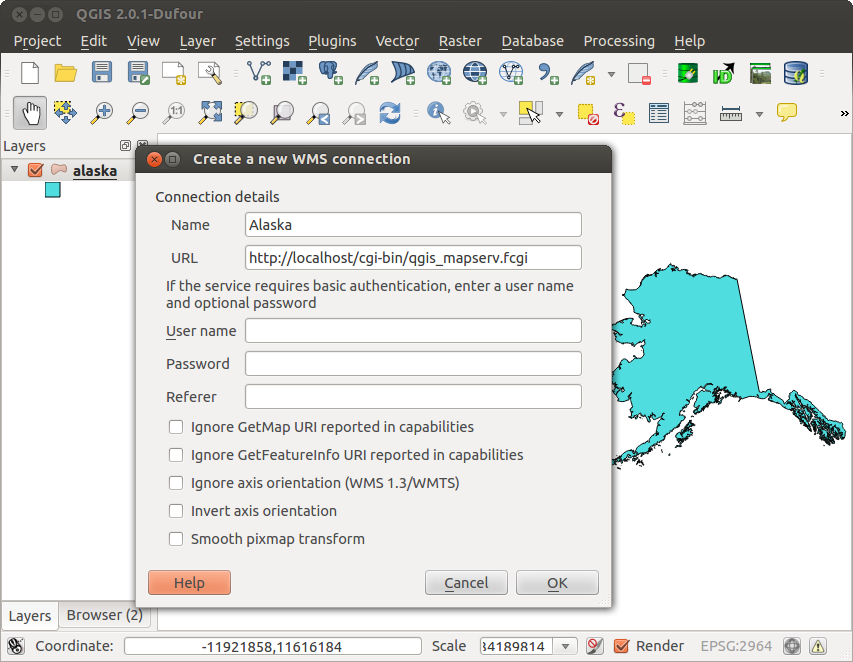
\includegraphics[clip=true, width=9cm]{standard_wms_usa}
%\caption{Standard WMS with USA boundaries included in the qgis server \nixcaption}
\caption{WMS standard montrant les frontières des USA inclus dans QGIS Server \nixcaption}
\label{fig:usa_wms}
\end{figure}

%\section{Creating a WMS from a QGIS project}
\section{Création d'un WMS depuis un projet QGIS}

%To provide a new qgis wms server we have to create a qgis project file with some data. Here we use the 'regions' and the 'aiport' shapefiles from the qgis\_sample\_dataset. 
Pour créer un nouveau serveur WMS QGIS, nous devons créer un fichier de projet QGIS avec quelques données. Nous utilisons ici les shapefiles des régions et des aéroports issus de qgis\_sample\_dataset.

%First load the shapefiles and define the colors and styles of the layers in QGIS and define the project CRS, if not already done. In a next step open the \tab{WMS Server} tab under \mainmenuopt{Settings} \arrow \mainmenuopt{Project Properties} and define the fields 'Service Capabilities', 'Coordinate System Restrictions' and 'Advertised Extend'. Additionally you can enable the checkbox \checkbox{Add WKT geometry to feature into response} to make the layers queryable (see figure \ref{fig:wmsdefinition}). Now save the session in a project file 'alaska\_airports.qgs'. 
Chargez tout d'abord les shapefiles, définissez les couleurs et styles des couches dans QGIS ainsi que le SCR du projet si ce n'est pas déjà fait. Ouvrez ensuite l'onglet  \tab{Serveur WMS} sous \mainmenuopt{Préférences} \arrow \mainmenuopt{Propriétés du projet}, cochez 'Capacités du serveur' et définissez les 'Restrictions du système de coordonnées', l''Emrpise annoncée'. Vous pouvez également cocher la case \checkbox{Ajouter une géométrie WKT à la réponse de l'entité} pour que les couches soient interrogeables (voir figure \ref{fig:wmsdefinition}). Sauvegardez enfin votre fichier de projet 'alaska\_airports.qgs'.

\begin{figure}[ht]
\centering
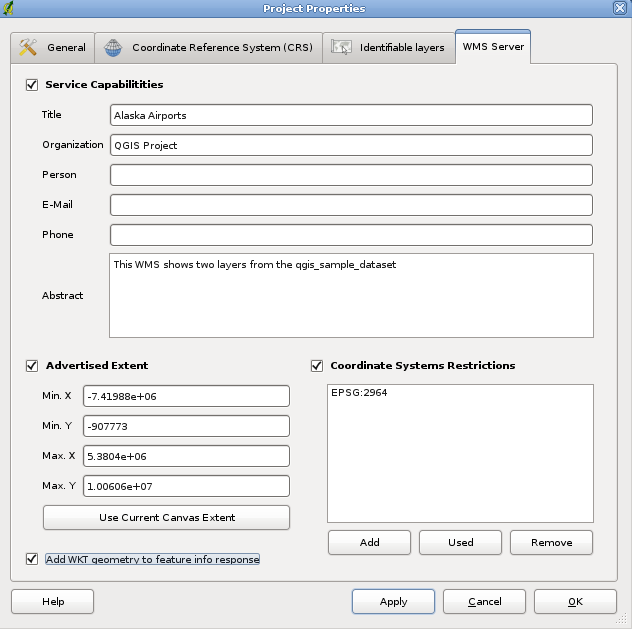
\includegraphics[clip=true, width=9cm]{wms_server_definition}
%\caption{Definitions for a qgis project WMS server \nixcaption}
\caption{Définition d'un projet de serveur WMS QGIS \nixcaption}
\label{fig:wmsdefinition}
\end{figure}

%To provide the project as a WMS, we create a new folder '/usr/lib/cgi-bin/project' with admin privileges and add the project file 'alaska\_airports.qgs' and a copy of the qgis\_mapserv.fcgi file - that's all.
Pour diffuser le projet en tant que WMS, créons un nouveau répertoire '/usr/lib/cgi-bin/project' avec les privilèges administrateur et ajoutons le fichier de projet 'alaska\_airports.qgs' ainsi qu'une copie du fichier qgis\_mapserv.fcgi - c'est tout.

%Now we test our project WMS, add the WMS with the URL http://localhost/cgi-bin/project/qgis\_mapserv.fcgi as described in section \ref{sec:ogc-wms-servers} to QGIS and load the WMS, see figure \ref{fig:wmsproject}.
Testons maintenant notre projet WMS. Ajoutez à QGIS la couche WMS venant de l'URL http://localhost/cgi-bin/project/qgis\_mapserv.fcgi tel que décrit dans la section \ref{sec:ogc-wms-servers} et chargez le WMS (voir figure \ref{fig:wmsproject}).

\begin{figure}[ht]
\centering
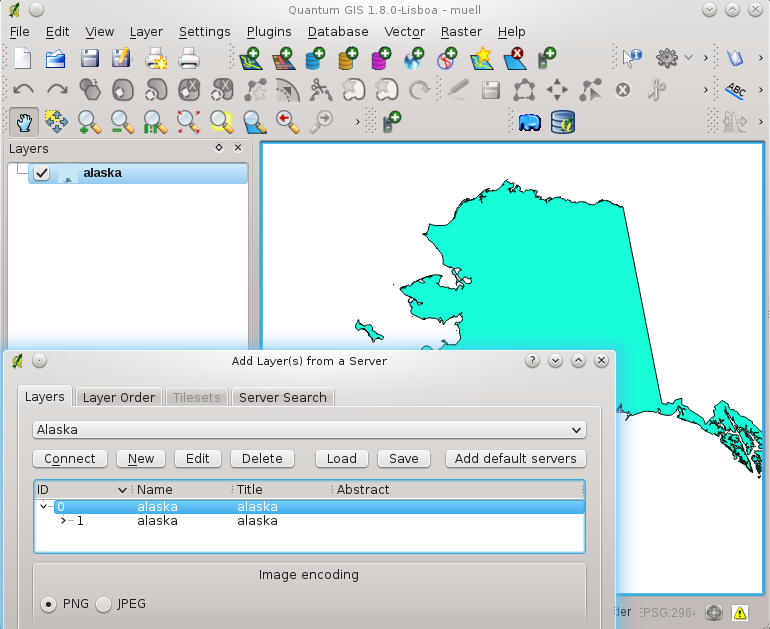
\includegraphics[clip=true, width=\textwidth]{wms_server_project}
%\caption{QGIS WMS Server based on a qgis project \nixcaption}
\caption{Serveur WMS QGIS basé sur un projet QGIS \nixcaption}
\label{fig:wmsproject}
\end{figure}

\FloatBarrier
